
% JuliaCon proceedings template
\documentclass{juliacon}
\setcounter{page}{1}

\usepackage{hyperref}
\usepackage[linesnumbered,ruled,vlined]{algorithm2e}
\usepackage{graphicx}
\usepackage[font=small,labelfont=bf]{caption}
\usepackage{subcaption}
\usepackage{todonotes}

\setlength{\parindent}{2em}
\setlength{\parskip}{1em}

% Change link color
\hypersetup{colorlinks=true}

\begin{document}

% **************GENERATED FILE, DO NOT EDIT**************

\title{RayTracer.jl: A General Purpose Differentiable Renderer}

\author[1]{Avik Pal}
\affil[1]{Indian Institute of Technology, Kanpur}

\keywords{Julia, Differentiable Programming, Deep Learning, Automatic Differentiation, Inverse Graphics}



\maketitle

\begin{abstract}
In this paper we present RayTracer.jl, a renderer in Julia that is fully differentiable using source-to-source Automatic Differentiation (AD). This means that RayTracer not only renders 2D images from 3D scene parameters, but it can be used to optimize for model parameters that generate a target image in a Differentiable Programming (DP) pipeline. We interface our renderer with the deep learning library Flux for use in combination with neural networks. We demonstrate the use of this differentiable renderer in rendering tasks and in solving inverse graphics problems.

\headingtable

\end{abstract}

% IMAGES

\begin{figure*}[!htb]
    \centering
    \begin{subfigure}[c]{0.45\textwidth}
        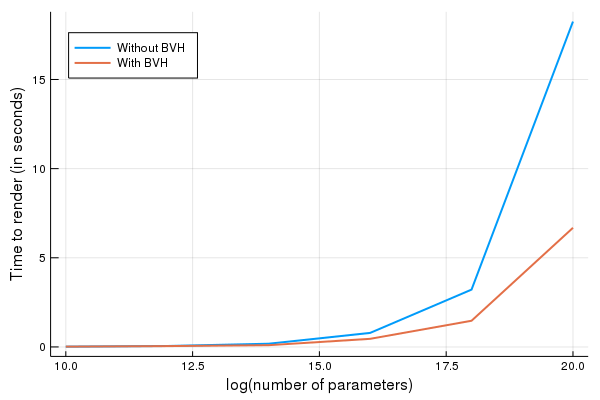
\includegraphics[height=75mm, width=\textwidth]{images/performance-speed.png}
        \caption{Performance Benchmarks}
        \label{fig:bvh_perf}
    \end{subfigure}
    \hfill
    \begin{subfigure}[c]{0.45\textwidth}
        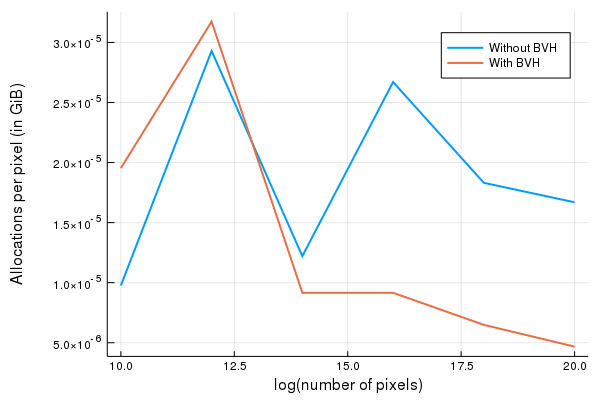
\includegraphics[height=75mm, width=\textwidth]{images/performance-memory.png}
        \caption{Memory Allocation Benchmarks}
        \label{fig:bvh_mem}
    \end{subfigure}
    \caption{Comparison between scenes rendered with and without BVH}
    \label{fig:bvh}
\end{figure*}

\begin{figure*}[!htb]
    \centering
    \begin{subfigure}[b]{0.3\textwidth}
        \centering
        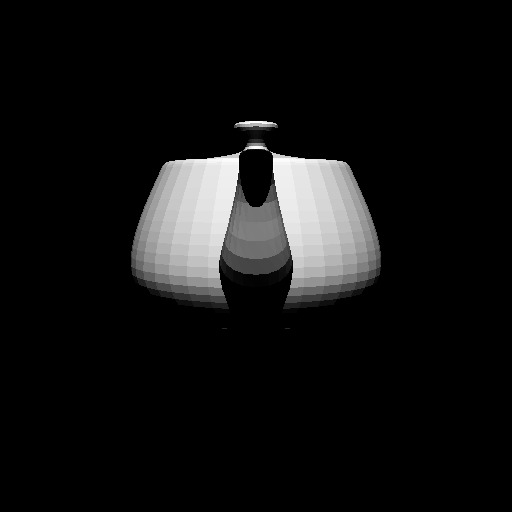
\includegraphics[width=\textwidth]{images/render/teapot_front.jpg}
        \caption*{}
    \end{subfigure}
    \hfill
    \begin{subfigure}[b]{0.3\textwidth}
        \centering
        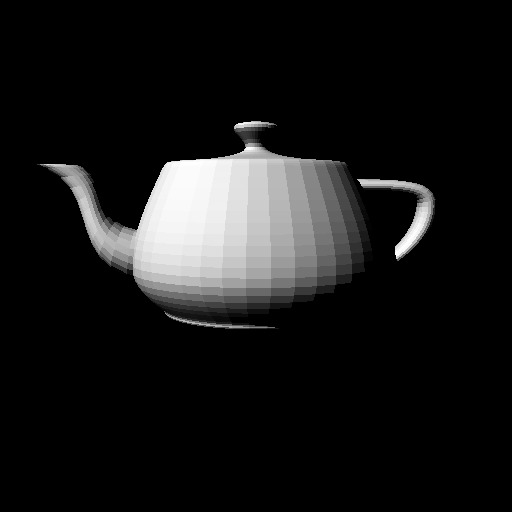
\includegraphics[width=\textwidth]{images/render/teapot_side.jpg}
        \caption*{}
    \end{subfigure}
    \hfill
    \begin{subfigure}[b]{0.3\textwidth}
        \centering
        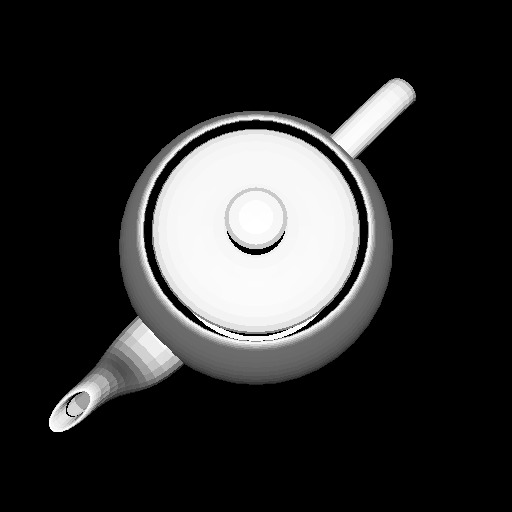
\includegraphics[width=\textwidth]{images/render/teapot_top.jpg}
        \caption*{}
    \end{subfigure}
    \caption{Utah Teapot Render from three different views. The camera definition shown in Listing~\protect\ref{lst:example_render} can be easily modified to generate all these views.}
    \label{fig:teapot_render}
\end{figure*}

\section{Introduction}
\label{intro}

Rendering is a technique of generating photorealistic or non photorealistic 2D projections from 3D objects. As such there are several algorithms for rendering complex scenes. One of the most popular techniques for photo realistic rendering is ray tracing. However, for real time rendering algorithms like rasterization are used.

Ray Tracing is a technique in computer graphics for rendering 3D graphics with complex light interactions. In this technique, rays are traced backwards from the eye/camera to the light source(s). The ray of can undergo reflection and refraction due to interactions with the objects in its path. This technique, however, is very computationally expensive and hence difficult to do in real time. But since ray tracing leverages the properties of the materials of the objects in the scene, a natural extension to the rendering problem would be to extract the exact properties of the materials, lighting, etc. given an image of the scene. Unfortunately ray tracing is non-differentiable at some points and calculating the analytic gradients is a very tedious task. This has made it a very difficult task to present a general inverse rendering method. As such there is only one framework in our knowledge, redner\cite{Li:2018:DMC}, which has been able to do so by using analytic gradients.

Rendering being a computationally expensive operation is generally done in static languages like C++. This makes it very time expensive to develop the software. Also, most languages lack the support of state of the art automatic differentiation tools like Zygote \cite{DBLP:journals/corr/abs-1810-07951}, Jax \cite{jax}, etc which are generally implemented for high level languages like Julia and Python. As such it is difficult to develop differentiable renderers in those languages and then interface with popular deep learning software.

In this paper, we explore the idea of differentiability through a renderer, by leveraging the AD in Julia\cite{bezanson2017julia}. We present a fully general renderer capable of handling complex scenes and able to differentiate through them. We don't rely on analytic gradients but use source-to-source AD to generate efficient gradient code in the backward pass.

\section{Differentiable Ray Tracing}

There are several photo-realistic renderers available which contain a vast amount of implicit knowledge. Differentiation allows such renderers to make use of gradients to learn the inverse mapping from an image to its parameter space. This knowledge can then be used in combination with any machine learning / deep learning models to train them in a fast and efficient manner. Experiments in \cite{retinaface} demonstrate the effectiveness of incorporate differentiable renderers in deep learning pipelines by achieving State of the Art results in WIDERFace Hard dataset.

However, as usual it is difficult to compute efficient derivatives from a production-ready renderer, typically written in a performance language like C++. This provides the primary motivation towards the development of RayTracer.jl. We develop an entire general purpose ray tracer in a high level numerical computation language. The presence of strong automatic differentiation libraries like Zygote.jl make it trivial to compute efficient derivatives from the renderer. We present the performance gains we get on using Zygote as compared to Central Differencing in Figure~\ref{fig:ad_perf}.

\begin{figure}[!htb]
    \centering
    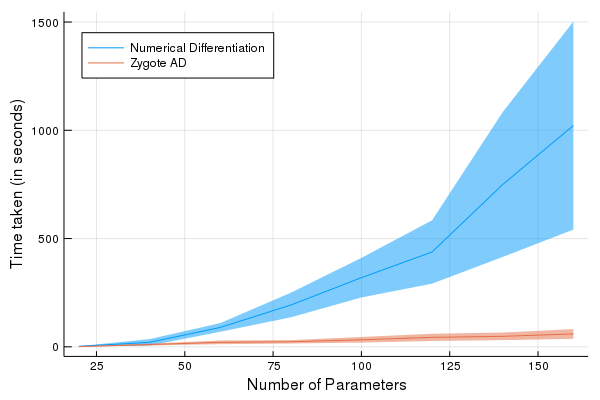
\includegraphics[width=\linewidth, height=150px]{images/differentiation.png}
    \caption{Performance Comparison between Zygote AD and Numerical Differentiation}
    \label{fig:ad_perf}
\end{figure}

RayTracer.jl \cite{RayTracer.jl} is a package for Differentiable Ray Tracing written to solve this particular issue. It relies heavily on the source-to-source automatic differentiation package, Zygote for computing gradients with respect to arbitrary scene parameters. This package allows the user to configure the location of objects, lights and a camera in the scene. This scene is then interpreted by the renderer to generate the image. RayTracer.jl is naturally interfaced with the deep learning library Flux \cite{Flux.jl-2018}, due to the common AD backend, for use in more complex differentiable pipelines.

\section{Scene Rendering}

Our approach to differentiable rendering is based on first creating a general purpose renderer and then make use of efficient AD tools for the differentiability part. Hence, at its core RayTracer is a fully featured renderer. It contains functionalities for both raytracing and rasterization. Additionally, unlike most prior work in differentiable rendering we do not make performance compromises in the forward pass (rendering) to allow gradient computation.

RayTracer gives users a lot of control to the user over the scene they want to render. The user controls the lighting in the scene, the shape and materials of the objects and the camera configuration.

\subsection{Accelerating the Rendering Process}

To accelerate the rendering process we have acceleration structures. Currently only one such acceleration structure, Bounding Volume Hierarchy \cite{Kay:1986:RTC:15922.15916}, is supported. We follow the exact same API for ray tracing using these accelerators. In this case instead of passing a \textit{Vector of Objects} we wrap it in a \textit{BoundingVolumeHierarchy} object and pass it. So in order to use this, we would have to change the scene variable to \textit{BoundingVolumeHierarchy(load\_obj("teapot.obj"))}.

\todo[inline]{Clarifications and Reproducibility}
We show the benefits of using Acceleration Structures in Figures~\ref{fig:bvh_perf} and \ref{fig:bvh_mem}. As can be seen from the plots we not only get a good performance gain (Figure~\ref{fig:bvh_perf}) in terms of speed, we also end up allocating much less memory (Figure~\ref{fig:bvh_mem} on using Bounding Volume Hierarchy.

\subsection{Rendering the Utah Teapot}
\todo[inline]{Clarity and Grammer}

In this section we shall render a very popular model in computer graphics: the Utah Teapot. We simply load the model from a wavefront object (obj) file. Support for other types of files is trivial through the MeshIO.jl package with defines file reader for common mesh object files. Once the scene is loaded the next step is to configure the other elements in the scene - the camera and the light(s). Script~\ref{lst:example_render} illustrates the code for rendering the teapot model.

\noindent
\begin{minipage}{\linewidth}
\begin{lstlisting}[caption = {Rendering the Utah Teapot Model},
                   label = {lst:example_render},
                   captionpos = b,
                   language = Julia]
# Screen Size
screen_size = (w = 512, h = 512)
    
# Camera Setup
cam = Camera(
    Vec3(1.0f0, 10.0f0, -1.0f0),
    Vec3(0.0f0),
    Vec3(0.0f0, 1.0f0, 0.0f0),
    45.0f0,
    1.0f0,
    screen_size...
)
                 
origin, direction = get_primary_rays(cam)
    
# Scene
scene = load_obj("teapot.obj")
    
# Light Position
light = DistantLight(
    Vec3(1.0f0),
    100.0f0,
    Vec3(0.0f0, 1.0f0, 0.0f0)
)
                         
# Render the image
color = raytrace(
    origin,
    direction,
    scene,
    light,
    origin,
    2
)
\end{lstlisting}
\end{minipage}

\section{Inverse Rendering}

\todo[inline]{More clarity in writing}

Just like rendering can be thought of as the projection of 3D objects into a 2D plane, the inverse rendering problem can be described as just the opposite. It is the mapping of the 2D image back to the parameters of the scene.

As we have mentioned previously, one of the primary motivations of RayTracer.jl is for solving the problem of inverse graphics. Being able to compute gradients wrt any scene parameter, means that we can optimize that parameter. The optimization algorithm is pretty straight forward and is general enough to work for any arbitrary parameter. We describe the algorithm in \ref{alg:inv_render}.

\begin{algorithm}[!htb]
    \caption{Gradient Based Optimization of Scene Parameters}
    \label{alg:inv_render}
    \SetAlgoLined
    \KwResult{Optimized set of Camera Parameters}
    Initial Guess of Parameters\;
    \While{not \textbf{converged} or iter < max\_iter}{
        gs = gradient(params) \textbf{do}\\
        ~~~~~~img = rendered image with params\;
        ~~~~~~loss = mean\_squared\_loss(img, target\_img)\;
        \textbf{end}\;
        \For{param in params}{
            update!(optimizer, param, gs[param])\;
        }
        \If{loss < tolerance}{
            converged = True\;
        }
    }
\end{algorithm}

\section{Experiments}

\begin{figure*}[!htb]
    \centering
    \begin{subfigure}[c]{0.26\textwidth}
        \centering
        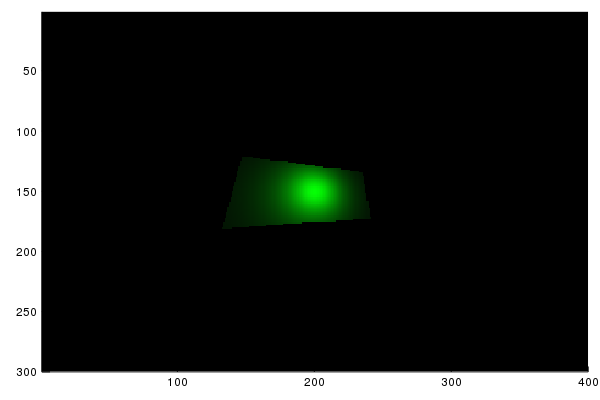
\includegraphics[width=107px, height=80px]{images/camera/initial_guess_image.png}
        \caption{Image with uncalibrated camera}
        \label{fig:cam_guess}
    \end{subfigure}
    \hfill
    \begin{subfigure}[c]{0.26\textwidth}
        \centering          
        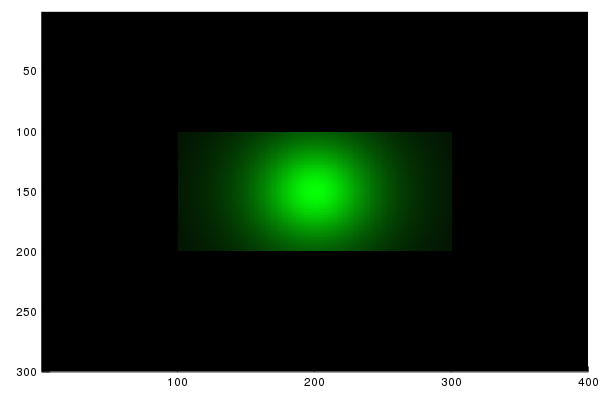
\includegraphics[width=107px, height=80px]{images/camera/target_image.png}
        \caption{Image to be reconstructed}
        \label{fig:cam_target}
    \end{subfigure}
    \centering
    \begin{subfigure}[c]{0.47\textwidth}
        \centering
        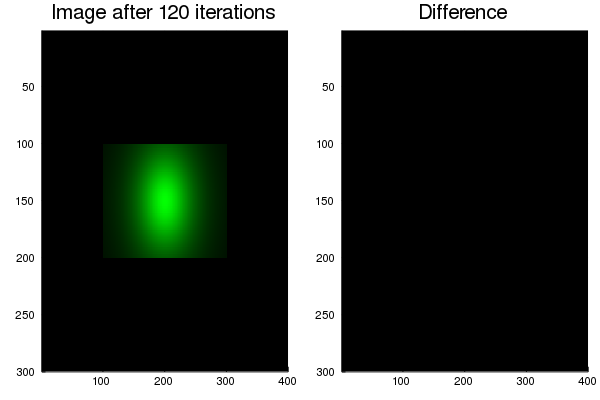
\includegraphics[width=\textwidth, height=80px]{images/camera/iter_120.png}
        \caption{Image obtained after optimization}
    \end{subfigure}
    \caption{Calibration of Camera Parameters to reconstruct Image~\ref{fig:cam_target} from Image~\ref{fig:cam_guess}}
    \label{fig:cam_invrender}
\end{figure*}

\begin{figure*}[!htb]
    \centering
    \begin{subfigure}[b]{0.45\textwidth}
        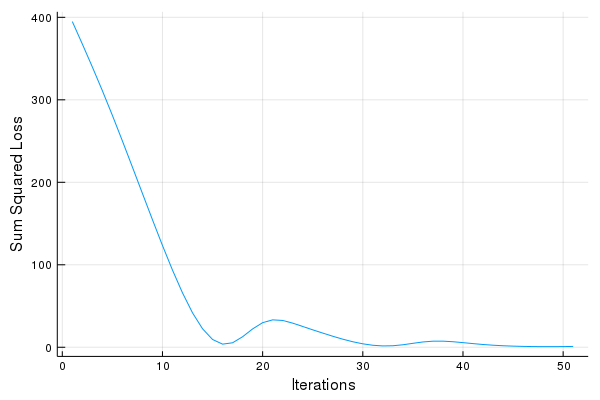
\includegraphics[width=\linewidth]{images/light/loss_plot_light.png}
        \caption{Loss Values over the Light Configuration Optimization Process}
        \label{fig:loss_plot_light}
    \end{subfigure}
    \hfill
    \begin{subfigure}[b]{0.45\textwidth}
        \begin{subfigure}[b]{0.4\textwidth}
            \centering
            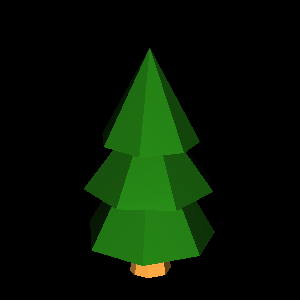
\includegraphics[width=\textwidth]{images/light/original.png}
            \caption{Image to be reconstructed}
            \label{fig:target_light}
        \end{subfigure}
        \hfill
        \begin{subfigure}[b]{0.4\textwidth}
            \centering
            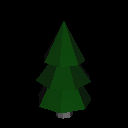
\includegraphics[width=\textwidth]{images/light/initial.png}
            \caption{Initial Guess of Lighting Parameters}
            \label{fig:guess_light}
        \end{subfigure}
        \centering
        \hfill
        \begin{subfigure}[b]{0.4\textwidth}
            \centering
            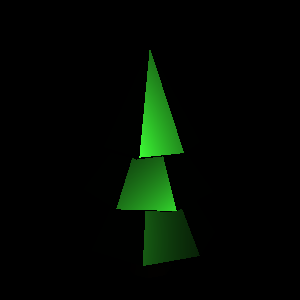
\includegraphics[width=\textwidth]{images/light/161.png}
            \caption{Image produced after 10 iterations}
        \end{subfigure}
        \hfill
        \begin{subfigure}[b]{0.4\textwidth}
            \centering
            
\includegraphics[width=\textwidth]{images/light/501.png}
            \caption{Image with converged parameters}
        \end{subfigure}
    \end{subfigure}
    \caption{Optimization of the lighting conditions to reconstruct Image~\ref{fig:target_light} from Image~\ref{fig:guess_light}}
    \label{fig:light_position}
\end{figure*}

In this section we showcase our differentiable renderer in some toy inverse rendering problems. Using the following two experiments we demonstrate the use of gradients obtained via AD to recover the camera and lighting parameters fr a scene. In both the experiments we make use of the Adam optimizer as described in \cite{kingma2014adam}. We interface the raytracer with Flux to use these optimizers. As an alternative, we have tested the functioning of our package with the optimizers present in Optim.

\subsection{\textbf{Calibration of Camera Parameters}}
\label{sec:calcam}

In this experiment we start with the image of a rectangle (Listing~\ref{lst:rect_light}) under some configuration of the Camera model (Listing~\ref{lst:cam_opt}). Since RayTracer supports only two primitive shapes - Spheres and Triangles, we need to triangulate the rectangle.

\noindent
\begin{minipage}{\linewidth}
\begin{lstlisting}[caption = {Configuration of the Rectangle for Experiment~\ref{sec:calcam}},
                   label = {lst:rect_light},
                   captionpos = b,
                   language = Julia]
scene = [
    Triangle(
        Vec3( 20.0,  10.0, 0.0),
        Vec3( 20.0, -10.0, 0.0),
        Vec3(-20.0,  10.0, 0.0),
        Material(
            color_diffuse = Vec3(0.0, 1.0, 0.0))),
    Triangle(
        Vec3(-20.0, -10.0, 0.0),
        Vec3( 20.0, -10.0, 0.0),
        Vec3(-20.0,  10.0, 0.0),
        Material(
            color_diffuse = Vec3(0.0, 1.0, 0.0)))
]
\end{lstlisting}
\end{minipage}

\noindent
\begin{minipage}{\linewidth}
\begin{lstlisting}[caption = {Camera Parameters to be Reconstructed},
                   label = {lst:cam_opt},
                   captionpos = b,
                   language = Julia]
camera_target =
    Camera(
        Vec3(0.0, 0.0, -30.0),
        Vec3(0.0, 0.0,   0.0),
        Vec3(0.0, 1.0,   0.0),
        90.0,
        1.0,
        screen_size...
    )
\end{lstlisting}
\end{minipage}

\noindent
\begin{minipage}{\linewidth}
\begin{lstlisting}[caption = {Light Configuration},
                   label = {lst:lgt_param},
                   captionpos = b,
                   language = Julia]
light = PointLight(
    Vec3(1.0, 0.0, 0.0),
    100000.0,
    Vec3(0.0, 0.0, -10.0)
)
\end{lstlisting}
\end{minipage}

Our aim is to reconstruct the image of this rectangle (Figure~\ref{fig:cam_target}) by modifying the focus and the location of the camera. We assume that all the other parameters of the model, like the light configuration (Listing~\ref{lst:lgt_param}), position of objects, etc. are known apriori. We use algorithm~\ref{alg:inv_render} for optimizing the parameters. We make an initial guess of the parameters and initialize the camera (Listing~\ref{lst:cam_initial}).

\noindent
\begin{minipage}{\linewidth}
\begin{lstlisting}[caption = {Initial Guess of the Camera Parameters},
                   label = {lst:cam_initial},
                   captionpos = b,
                   language = Julia]
camera_guess =
    Camera(
        Vec3(5.0, -4.0, -20.0),
        Vec3(0.0,  0.0,   0.0),
        Vec3(0.0,  1.0,   0.0),
        90.0,
        3.0,
        screen_size...
    )
\end{lstlisting}
\end{minipage}

As our loss function, we use the mean squared difference between rendered and target images, each with $300\times400$ pixels having fractional RGB values. We minimize loss with the Adam optimizer, with learning rate 0.05, and declare the model to have converged if loss falls below 10 (where the initial loss is in the order of 600). Figure~\ref{fig:cam_invrender} shows the optimization steps.

\subsection{\textbf{Optimizing the Light Source}}
\todo[inline]{More details to reproduce the results}

In this experiment we describe our solution to the inverse lighting problem. In this case we assume the knowledge of the geometry and surface properties of the objects, camera position and the target image of the scene.

For this experiment we try to optimize the lighting for a scene containing a tree. We are given the target image with proper lighting conditions. We start with an arbitrary lighting and then iteratively improve the lighting using algorithm~\ref{alg:inv_render}.

We present the images generated during the optimization process in Figure~\ref{fig:light_position}.

\section{Current Limitations}
\todo[inline]{Write this section highlighting the problem for non differentiable parts}


\section{Conclusion}
\todo[inline]{Needs a rewrite using the comments in the review}
In conclusion, we have presented how julia can be leveraged to build differentiable systems. Integrating them with the machine learning pipeline can make an end-to-end differentiable pipeline. Using this pipeline we can define differentiable programming algorithm on it to solve the problem. As expected making the pipeline differentiable allows us to exploit the huge amount of implicit knowledge stored in the system.

% \newpage

\bibliographystyle{juliacon}
\bibliography{ref}

\end{document}

% Inspired by the International Journal of Computer Applications template

